\chapter[Learning with Unknown Input Observers for Robust Nonlinear Estimation]{Learning with Unknown Input Observers for Robust Nonlinear Estimation}\label{chp4_chap}
\chaptermark{Learning with Unknown Input Observers for Robust Nonlinear Estimation}

\objectif{This chapter introduces a robust hybrid state estimation framework for vehicle motion tracking that combines physics-based guarantees with data-driven adaptability. Standard model-based observers often fail when strict rank conditions are not met, while pure neural network approaches lack stability guarantees. To address this, we propose a two-stage architecture. First, we develop a Generalized Unknown Input Observer (UIO) that utilizes output derivatives to relax the standard rank condition, ensuring the existence of a bounded estimation of unmodeled dynamics. Second, we introduce a Neural Adaptive Observer that treats the UIO estimates as a "teacher" signal. Unlike the UIO, which provides instantaneous signal estimation, the neural observer learns the underlying structure of the uncertainty as a function of the state. This allows the system to predict disturbances along reference trajectories and refine the estimation error asymptotically. The approach is validated via Linear Matrix Inequalities (LMIs) ensuring $\mathcal{H}^{1}$ and $\mathcal{L}_{2}$ stability.
}

%%%%%%%%%%%%%%%%%%%%%%%%%%%%%%%%%%%%%%%%%%%%%%%%%%%%%%%%%%%%%%%%%%%%%%%%%%%%%%%%%%%%%%%%%%%%%%%%%
\section{Introduction}


State estimation is a cornerstone of autonomous vehicle control, where safety depends on accurate knowledge of system states and external disturbances. Traditional methods rely on explicit physics-based models \citep{State_Esti2017}. However, in vehicle dynamics, highly nonlinear phenomena-such as variable tire-road friction or aerodynamic drag are difficult to model mathematically, leading to estimation errors that compromise control performance.

Data-driven methods, particularly Neural Networks (NNs), have emerged as powerful tools for approximating these complex nonlinear functions \citep{2006Apdat, HO_GP}. While NNs offer superior adaptability, they pose significant risks in safety-critical applications. In online learning scenarios, small shifts in input data can cause NNs to behave unpredictably or diverge, lacking the stability guarantees provided by control theory. Consequently, recent research has shifted toward hybrid architectures that embed learning within observer frameworks.

A major limitation in existing hybrid observers is their reliance on the standard observer matching condition. For many vehicle systems, this condition does not hold, making it theoretically impossible to decouple the unknown input from the state using standard techniques. While some methods attempt to bypass this using approximations, they often result in unbounded errors or require expensive additional sensors.

To overcome these limitations, this paper proposes a layered Teacher-Student estimation architecture consisting of two distinct observers:
\begin{itemize}
    \item  A Generalized UIO (The Teacher): We introduce a regularization technique using output derivatives that ensures the observer exists even when the rank condition fails. This observer provides a robust, physics-guaranteed signal of the unknown input, ensuring the estimation error remains bounded. 
    
    % The generalized UIO does not rely on numerical differentiation of outputs. Instead, it augments the system with output-derivative states, which are either directly measured (e.g., via IMU sensors) or internally estimated by the observer, thereby increasing output richness and enabling unknown-input reconstruction even when classical rank conditions fail.
    \item A Neural Adaptive Observer (The Student): While the UIO estimates the current value of the disturbance, it cannot predict how that disturbance behaves at future states (e.g., along a reference trajectory). The Neural Observer utilizes the UIO's signal to learn the unknown dynamics as a function of the state ($\mu_\theta(x)$). This allows for refined precision and enables the controller to anticipate unmodeled dynamics.
\end{itemize}
This combination offers a specific advantage: the Generalized UIO guarantees the system never diverges (safety), while the Neural Network minimizes the residual error over time (performance). The contributions of this paper are:
\begin{itemize}
    \item A Generalized UIO design that relaxes the rank condition using output derivatives ;
    \item A hybrid learning framework where the UIO acts as a supervisor, enforcing consistency in the neural training loop; 
    \item LMI-based stability conditions that guarantee joint convergence of both the state and model parameters. 
\end{itemize}




%%%%%%%%%%%%%%%%%%%%%%%%%%%%%%%%%%%%%%%%%%%%%%%%%%%%%%%%%%%%%%%%%%%%%%%%%%%%%%%%%%%%%%%%%%%%%%%%%
\section{Problem Formulation and Motivation}\label{sec2}
%
In this paper, we consider the class of continuous-time nonlinear systems in state-space form described by the following equations:

\begin{equation}\label{sys_1}
    \begin{array}{l}
        \dot{x} = \varphi(x,u) + B\mu_{x}  \\
        y = Cx, 
    \end{array}
\end{equation}
where $x\in \mathcal{X} \subseteq\mathbb{R}^{n_x}$ is the state vector, $y\in\mathbb{R}^{n_y}$ is the output measurement, $u\in\mathcal{U} \subseteq\mathbb{R}^{n_u}$ is the control input, and $\mu_{x}\in\mathbb{R}^{n_{\mu}}$ is an unknown nonlinear function that encapsulates the system uncertainty including both unmodeled dynamics and external disturbances. The matrices $C\in\mathbb{R}^{n_y}\times\mathbb{R}^{n_x}$ and $B\in\mathbb{R}^{n_x}\times\mathbb{R}^{n_{\mu}}$ are constant and known matrices. The function $\varphi: \mathcal{X} \times \mathcal{U} \to \mathbb{R}^{n_x}$ represents the known nonlinear component of the system. 

\begin{remark}
For simplicity, we consider systems with linear output. Otherwise, if we have nonlinear output $y = h(x)$, we introduce a new state $\eta(t)$, with $\dot{\eta} \triangleq A_{\eta} \eta + \gamma y$ and $\eta_0 = \eta(0)$ known. Then, a new system with the augmented vector $\zeta = \begin{bmatrix} \eta \\ x \end{bmatrix}$ may be considered, which has as linear output the vector $\eta$.
\end{remark}


Now, let us introduce the following assumptions which are required for our unknown input observer design methods.
\begin{assumption}\label{ali_hyp1}
%Assumption 1. 
The output vector $y$ has dimension greater than or equal to the number of unknown terms~$\mu_{x}$; equivalently, $n_{\mu} \leq n_y$.
\end{assumption}

\begin{assumption}\label{ali_hyp2}
%Assumption 2. 
The nonlinear function $\varphi(.)$ is $\gamma_{\varphi}-$Lipschitz continuous on $\mathcal{X}$, uniformly on $u\in\mathcal{U}$.
\end{assumption}

\begin{assumption}\label{ali_hyp3}
The unknown nonlinearity $\mu_{x}(.)$ is Lebesgue measurable and $\mathcal{L}_{2}-$bounded.
\end{assumption}


{\color{blue}
\begin{remark}
Assumption~\ref{ali_hyp3} corresponds to a \emph{bounded-energy} uncertainty over $\Omega=[0,+\infty[$, which is standard in $\mathcal{H}_{\infty}$/\,$\mathcal{L}_{2}$-gain observer analysis. In the vehicle context, $\mu_x$ may represent aggregated effects such as unmodeled tire-force nonlinearities, residual parameter mismatches, aerodynamic disturbances, or actuator/sensor fault components.
Moreover, since the regularization introduced later contains $\omega_{\delta_{1}}(t)=\delta_1\dot{\mu}_x(t)$, the subsequent $\mathcal{H}^1$ performance bound implicitly requires $\mu_x\in\mathcal{H}^1(\Omega)$ (i.e., $\mu_x\in\mathcal{L}_2(\Omega)$ and $\dot{\mu}_x\in\mathcal{L}_2(\Omega)$), which can be interpreted as \emph{bounded-energy variations} of the unknown input.
\end{remark}
}


The objective of this paper is to estimate the unmodeled dynamics $\mu_{x}$. More specifically, we propose to estimate $\mu_{x}$ by combining an unknown input observer~(UIO) with a neural network--based approach, leveraging gradient-based methods to better capture the unmodeled components of the system. The key idea is to incorporate the UIO-based estimation into the loss function of the neural network, thereby enhancing residual regularization and ensuring consistency with the UIO. This, in turn, improves the robustness and performance of the overall estimation scheme. Unfortunately, it is not possible to estimate the unknown input, $\mu_x$, if the system fails to satisfy the following main necessary condition:
\begin{equation}\label{rank}
\textrm{rank}(C B) = \textrm{rank}(B).
\end{equation}
%
In addition, to be able to directly construct a UIO for system~\eqref{sys_1} to estimate simultaneously $x$ and $\mu_x$, the constraint~\eqref{rank} is not sufficient. For this, we should be able to write the system under the form:
\begin{equation}\label{sys_2}
    \begin{array}{l}
        \mathbb{E} \dot{\zeta} = \varphi_{\zeta}(\zeta,u)  \\
        y = \mathcal{H} \zeta
    \end{array}
\end{equation}
with
\begin{equation}\label{rank2}
\textrm{rank}\left( \begin{bmatrix} \mathbb{E} \\  \mathcal{H} \end{bmatrix} \right) = n_{x} + n_{\mu}.
\end{equation}
%--
For further details on this requirement, the reader is referred to~\cite{chaouche2022unknown,trinh2011functional,Zemouche-Boutayeb-2009,Hassan13a,Trinh:TAC08} and the references therein. 

% % %%% Simple details of problem

% Various techniques address the rank condition issue. Some invert system dynamics [13]–[15] or rely on output derivatives [13], [16], which amplifies noise. Others augment the system with additional sensors [13], which increases cost. Proportional-Integral Observers (PIO) often assume null dynamics [17], [18] or constant inputs [19], which is overly conservative for vehicle dynamics. 
% % %%% Simple details of problem


%%% TOO much details of the literature
To address this challenge, various techniques have been proposed in the literature, each offering a different approach to the problem. Without aiming for exhaustiveness, these techniques can be summarized as follows. Nevertheless, the problem remains open, and new ideas or improvements are still possible, although often at the cost of additional assumptions:
%==
\begin{itemize}
\item {\it Inverting the system dynamics:} The system state is first estimated, and the unknown inputs are then obtained by inverting the dynamics~\cite{Phanomchoeng:ASME/TM14,Benallouch:TCST17,Marquez:Auto14}. However, the presence of disturbances and nonlinearities in the output signal or in the dynamics can make the problem particularly challenging.
%



\item {\it Deriving the output vector $y(t)$:} In some cases, the derivatives of the output measurements are required~\cite{Hou:256351,Phanomchoeng:ASME/TM14}. This leads to the construction of a pseudo-output vector $y_{\rm new}$, which enables the simultaneous estimation of $x$ and $\mu_{x}$. For instance, in the linear case without disturbances, one obtains 
$$
y_{\rm new} = C_{\rm new} x + C_{\mu}\mu_{x},
$$
where $\mathrm{rank}(C_{\mu}) = n_{\mu}$. However, this approach is not suitable for nonlinear disturbed systems, since differentiating $y(t)$ introduces additional variables arising from the derivatives of the disturbance vector, as well as new nonlinearities in the pseudo-output vector. Consequently, satisfying the rank condition~\eqref{rank} with the new matrices becomes very difficult.

%
\item {\it Adding sensors:} In some cases, augmenting the system with additional sensors is a natural way to overcome the rank condition~\eqref{rank}. This approach introduces a new measurement vector $y_{\rm new}$, where the original output $y(t)$ is used to estimate the state $x(t)$, and the additional outputs $y_{\rm new}$ are exploited to estimate the unknown input, $\mu_{x}$. For example, in~\cite{Phanomchoeng:ASME/TM14} (and references therein), four sensors (i.e., four output measurements) were employed to estimate only two unknown inputs. However, the presence of disturbances can significantly decrease estimation performance. Moreover, additional sensors may be very expensive or, in some cases, unavailable.
%
\item {\it Proportional--Integral Observer and Null Dynamics:} Some works in the literature have employed a Proportional--Integral Observer (PIO) together with null dynamics imposed on the estimated unknown input~\cite{PIO_1995,PIOreview}. However, this assumption does not reflect the true dynamics of the unknown input, leading to inaccurate estimation. Other approaches assume constant inputs~\cite{jeon2020simultaneous}, i.e., $\dot{\mu}_{x} \equiv 0$, but this restriction is overly conservative. Recently, a method for discrete-time systems was proposed in~\cite{nguyen2024cyberattack}; however, this approach yields delayed estimates of both the system state and the unknown inputs, which is often impractical to design reliable controllers.
\end{itemize}
%%%%

The limitations of the aforementioned methods motivated us to adopt a different approach and propose a simple strategy to estimate the system state and the unknown input without relying on conservative assumptions. The key idea is to recognize that this initial estimation is not final. Rather, the objective is to provide a first-level approximation of $x$ and $\mu_{x}$, which will subsequently be refined through the neuro-adaptive observer we introduce later. This refinement enhances estimation accuracy and ultimately yields a definitive estimate of the unmodeled nonlinearity, $\mu_{x}$.


The strategy consists in rewriting system~\eqref{sys_1} without modifying it. Then, the UIO we will propose will be based on reliable approximation of~\eqref{sys_1}.

\begin{equation}\label{ali_syst1}
    \begin{array}{l}
        \dot{x} + E_{\delta_1} \dot{\mu}_{x} = \varphi(x,u) + B\mu_{x} + E \omega_{\delta_{1}} \\
        y = Cx + D_{\delta_2} \mu_{x} + D\, \omega_{\delta_{2}} 
    \end{array}
\end{equation}
where $D \in \mathbb{R}^{n_y \times n_{\mu}}$ and $E \in \mathbb{R}^{n_x \times n_{\mu}}$ are given constant, full-column-rank matrix specified by the user; $E_{\delta_1} = \delta_{1} E, D_{\delta_2} = \delta_{2} D$; and $\omega_{\delta_{1}}(t) = \delta_{1} \dot{\mu}_{x}(t), \omega_{\delta_{2}}(t) = \delta_{2} \mu_{x}(t)$, with $\delta_{j} \geq 0$, with $(\delta_1,\delta_2) \neq (0,0)$, chosen sufficiently small to ensure the feasibility of some sufficient conditions that will be stated later. The purpose of this reformulation is to recover the rank condition~\eqref{rank2}, at the expense of introducing the additive terms $\omega_{\delta_{j}}(t), j=1,2$, which are handled as disturbances. 

{\color{blue}
\begin{itemize}
    \item \textbf{Design guideline for $E$ and $D$:} in practice, $E$ and $D$ can be selected as sparse (often binary) full-column-rank matrices that \emph{inject} the regularization terms into a subset of state/output channels so that the augmented pair $(\mathbb{E},\mathcal{H})$ satisfies Assumption~\ref{ali_hyp4}. A simple procedure is to (i) choose $D$ so that $\mathrm{rank}(D)=n_{\mu}$ (typically by selecting $n_{\mu}$ independent measured outputs), and then (ii) choose $E$ (possibly also sparse/binary) to complete the rank condition~\eqref{rank2} with minimal additional coupling.
    \item \textbf{Interpretation of $\delta_1,\delta_2$:} the scalars $\delta_1$ and $\delta_2$ quantify the trade-off between \emph{rank recovery} (feasibility of Assumption~\ref{ali_hyp4}) and \emph{disturbance amplification} through the induced terms $\omega_{\delta_1}$ and $\omega_{\delta_2}$.
\end{itemize}
}
The next section presents LMI conditions that guarantee accurate estimation of $x$ and $\mu_{x}$ while satisfying an $\mathcal{H}_{\infty}$ criterion, or more specifically, an $\mathcal{L}_{2}$-optimality criterion---where the performance bound is proportional to $\delta_{j}, j=1,2$.








\section{LMI-Based $\mathcal{H}^{1}$ UIO Design}\label{uio}
%==  $\mathcal{W}^{1,2}$
This section is devoted to the numerical LMI-based design procedure ensuring the asymptotic estimation of the system state $x$ and the unmodeled dynamics $\mu_{x}$ following a $\mathcal{H}^{1}-$optimality criterion.

%===========
\subsection{System transformation}
%-----
Recall that $\mathcal{H}^{1}$ is the {\it Hilbert} space corresponding to the {\it Sobolev} space, $\mathcal{W}^{1,2}$, of square--integrable functions whose weak first derivatives are also square--integrable. Mathematically, we define the set $\mathcal{H}^{1}\left( \Omega \right)$ as
$$
\mathcal{H}^{1}\left( \Omega \right) := \left\{ \psi \in \mathcal{L}^{2}(\Omega) \;\middle|\; \frac{\textrm{d} \psi}{\textrm{d} t} \in \mathcal{L}^{2}(\Omega) \right\}
$$
with $\Omega = [0~+\infty[$ in our case. This space is endowed by the norm $\| . \|_{\mathcal{H}^{1}}$ defined as follows:
$$
\| \psi \|_{\mathcal{H}^{1}} :=
\left( \| \psi \|_{\mathcal{L}^{2}}^2 + \left\| \frac{\textrm{d} \psi}{\textrm{d} t} \right\|_{\mathcal{L}^{2}}^2 \right)^{1/2}.
$$

First, system~\eqref{ali_syst1} can be rewritten under the compact form:
\begin{equation}\label{ali_syst2}
    \begin{array}{l}
        \mathbb{E} \dot{\zeta} = \varphi_{\zeta}(\zeta,u) + \bar{E} \bm{\omega}_{\delta} \\
        y = \mathcal{H} \zeta + \bar{D} \bm{\omega}_{\delta}
    \end{array}
\end{equation}
where
\begin{subequations}\label{ali_syst2_e1}
\begin{equation}\label{ali_syst2_e1_1}
\mathbb{E} := \begin{bmatrix} \mathbb{I}_{n_x} & E_{\delta_1} \end{bmatrix},~\mathcal{H} := \begin{bmatrix} C & D_{\delta_2} \end{bmatrix},
\end{equation}
%
\begin{equation}\label{ali_syst2_e1_2}
\bar{E} := \begin{bmatrix} E & 0_{n_{x}\times n_{\mu}} \end{bmatrix},~\bar{D} := \begin{bmatrix} 0_{n_{y}\times n_{\mu}} & D \end{bmatrix},
\end{equation}
%
\begin{align}\label{ali_syst2_e1_3}
\zeta := \begin{bmatrix} x \\ \mu_{x} \end{bmatrix},~\bm{\omega}_{\delta} := \begin{bmatrix} \omega_{\delta_{1}} \\ \omega_{\delta_{2}} \end{bmatrix},
\end{align}
%
%\vspace{-0.7cm}
\begin{align}\label{ali_syst2_e1_4}
\varphi_{\zeta}(\zeta,u) := \varphi(x,u) + B \mu_{x}.
\end{align}
\end{subequations}
%==
%
Now, let us introduce the following necessary assumption:
\begin{assumption}\label{ali_hyp4}
The matrices $E$ and $D$ are chosen such that $\mathbb{E}$ and $\mathcal{H}$ satisfy the rank condition~\eqref{rank2}.
\end{assumption}

The objective is to design a state observer that provides an estimate $\hat{\zeta}$ of $\zeta$, such that the following $\mathcal{H}^1$-optimality inequality holds:
%
\begin{align}%\label{ali_h1_e1}
\| \tilde{\zeta} \|_{\mathcal{H}^{1}} &\leq \lambda_{\delta} \, \left\| \mu_{x} \right\|_{\mathcal{H}^{1}}  + \beta \, \left\| \xi_0 \right\| \label{ali_h1_e1_2}
\end{align}
where $\tilde{\zeta} := \zeta - \hat{\zeta}$, $\lambda_{\delta}$ is the disturbance attenuation level, explicitly depending on $\delta_1$ and $\delta_2$, $\beta > 0$ is a weighting real constant, and $\xi_0$ is a vector depending on $\tilde{\zeta}(0)$ and $\mu_{x}(0)$.%$\mathcal{N}\left(\tilde{\zeta}(0), \mu_{x}(0)\right)$. $\xi_0 := \tilde{\zeta}(0) - D \mu_{x}(0)$
%--
%===========
\subsection{UIO structure and error dynamics}
%-----
From Assumption~\ref{ali_hyp4},  there exist two matrices $P_{\zeta}$ and $Q_{\zeta}$ such that
\begin{equation}\label{ali_syst2_e2}
 P_{\zeta} \mathbb{E} + Q_{\zeta} \mathcal{H} = \mathbb{I}_{n_{\zeta}}.
\end{equation}
where $n_{\zeta} := n_{x} + n_{\mu}$. These matrices are exploited in the following observer structure:
\begin{equation}\label{ali_syst2_e3}
\left\{
\begin{array}{rcl}
\dot{\eta} & = & P_{\zeta} \varphi_{\zeta}(\hat{\zeta},u) + K \left( y - \mathcal{H} \hat{\zeta} \right)
\\
\hat{\zeta} & = & \eta + Q_{\zeta} y 
\end{array}
\right.
\end{equation}
where $\hat{\zeta}$ is the estimate of $\zeta$ and $K \in\mathbb{R}^{n_{\zeta}}\times\mathbb{R}^{n_y}$ is the observer gain to be determined such that the estimation error, $\tilde{\zeta} : = \zeta - \hat{\zeta}$, satisfies the $\mathcal{H}^1$-optimality criterion~\eqref{ali_h1_e1_2} with appropriate $\lambda_{\delta}, \beta$, and $\xi_0$.
%

We have 

\begin{align}\label{ali_syst2_e4}
\tilde{\zeta} &= \zeta - \eta - Q_{\zeta} y \notag \\
&= \left(\mathbb{I}_{n_{\zeta}} - Q_{\zeta} \mathcal{H}\right) \zeta - \eta - Q_{\zeta} \bar{D} \bm{\omega}_{\delta} \notag \\
&\overbrace{ \mathrel{\scalebox{2}[1]{=}} }^{\eqref{ali_syst2_e2}} P_{\zeta} \mathbb{E} \zeta - \eta - Q_{\zeta} \bar{D} \bm{\omega}_{\delta}
\end{align}
which gives equivalently
\begin{equation}\label{ali_syst2_e5}
\overbrace{ \tilde{\zeta} + Q_{\zeta} \bar{D} \bm{\omega}_{\delta} }^{\xi(t)} = P_{\zeta} \mathbb{E} \zeta(t) - \eta(t).
\end{equation}
It is worth noting that the reformulation~\eqref{ali_syst2_e5} conveniently avoids the derivative of $\bm{\omega}_{\delta}$ in the derivation of the error dynamics.

By using the dynamics~\eqref{ali_syst2} and~\eqref{ali_syst2_e3}, we obtain
\begin{align}\label{ali_syst2_e6}
\dot{\xi} &= P_{\zeta} \left[ \varphi_{\zeta}(\zeta,u) - \varphi_{\zeta}(\hat{\zeta},u) \right] -K \mathcal{H} \tilde{\zeta} \notag \\
&\quad + \left(P_{\zeta} \bar{E} - K \bar{D} \right) \bm{\omega}_{\delta} \notag \\
&= \left(P_{\zeta} \nabla^{\varphi_{\zeta}}_{\zeta}(\bm{z},u) - K  \mathcal{H} \right) \xi \notag \\
&\quad+ \Big( \mathcal{E}\left( \bm{z},u\right) - K  \mathcal{D} \Big) \bm{\omega}_{\delta}
\end{align}
where
$$
\mathcal{E}\left( \bm{z},u\right) := \bar{E} - P_{\zeta} \nabla^{\varphi_{\zeta}}_{\zeta}(\bm{z},u) Q_{\zeta} \bar{D}
$$
%==
$$
\mathcal{D} := \left( \mathbb{I}_{n_y} + \mathcal{H} Q_{\zeta} \right) \bar{D}.
$$
and from the differential mean value theorem~\cite{Hasni_LCSS_24}, we have
$$
\varphi_{\zeta}\left(\zeta,u \right) - \varphi_{\zeta}\left(\hat{\zeta},u \right) = \nabla^{\varphi_{\zeta}}_{\zeta}(\bm{z},u) \tilde{\zeta}
$$
for a given $\bm{z}$.

From this point onward, the analysis will be carried out with the vector~$\xi$ instead of~$\tilde{\zeta}$, and we will return to~$\tilde{\zeta}$ at the end to derive the final $\mathcal{H}^{1}$ bound~\eqref{ali_h1_e1_2}.
%===========
\subsection{New LMI-based UIO design conditions}
%-----
Before presenting the proposed LMI-based UIO design procedure, we state an intermediate and general result in the following proposition.
%-
\begin{proposition}\label{ali_prop1}
Le $\vartheta(.)$ be a Lyapunov function such that there exists $\vartheta_{\max} >0$ such that $\vartheta(z) \leq \vartheta_{\max}\| z \|^{2}$, for all $z \in \mathbb{R}^{n_\zeta}$. Consider a matrix $\mathcal{S} = \mathcal{S}^{\top} > 0$ and a real constant $\lambda >0$ such that the following inequality holds:
\begin{equation}\label{ali_prop1_e1}
\dot{\vartheta}(z) + \| z \|^{2} + \dot{z}^{\top} \mathcal{S} \dot{z} - \lambda \| w \|^{2} \leq 0,
 \forall z \in \mathbb{R}^{n_\zeta}, w \in \mathbb{R}^{2n_{\mu}}
\end{equation}
%
with $z \in \mathcal{H}^{1}$ and $w \in \mathcal{L}^{2}$. Then, the following inequality is satisfied:
\begin{equation}\label{ali_prop1_e2}
\| z \|_{\mathcal{H}^{1}} \leq \sqrt{\frac{\lambda}{\min\left(1,\lambda_{\min}(\mathcal{S})\right)}} \| w \|_{\mathcal{L}^{2}}  
+\sqrt{\frac{\vartheta_{\max}}{\min\left(1,\lambda_{\min}(\mathcal{S})\right)}} \| z_0 \|.
\end{equation}
Moreover, if~\eqref{ali_prop1_e1} is satisfied with $z := \xi$ and $w := \bm{\omega}_{\delta}$, where $\xi$ and $\bm{\omega}_{\delta}$ are defined by~\eqref{ali_syst2_e5} and~\eqref{ali_syst2_e1_3}, respectively, then the estimation error, $\tilde{\zeta}$, satisfies the $\mathcal{H}^{1}$ bound~\eqref{ali_h1_e1_2} with $\lambda_{\delta}$, $\beta$, and $\xi_0$ given as follows:
\begin{subequations}
\begin{equation}\label{ali_prop1_e3}
\lambda_{\delta} := \delta_{2} \sigma_{\max}\left(Q_{\zeta} D\right) 
+ \max\left(\delta_{1}, \delta_{2} \right) \sqrt{\frac{\lambda}{\min\left(1,\lambda_{\min}(\mathcal{S})\right)}}
\end{equation}
%--
\begin{equation}\label{ali_prop1_e4}
\beta := \sqrt{\frac{\vartheta_{\max}}{\min\left(1,\lambda_{\min}(\mathcal{S})\right)}}
\end{equation}
%--
\begin{equation}\label{ali_prop1_e5}
\xi_0 := \tilde{\zeta}(0) + Q_{\zeta} D \mu_{x}(0).
\end{equation}
\end{subequations}
where $\sigma_{\max}\left(Q_{\zeta} D\right)$ represents the largest singular value of the matrix $Q_{\zeta} D$.
\end{proposition}
%==
\begin{proof}
The first part of the proof is relatively straightforward. Before integrating~\eqref{ali_prop1_e1} to get the norms $\| . \|_{\mathcal{H}^{1}}$ and $\| . \|_{\mathcal{L}^{2}}$, take in mind that
$$
\min\left(1,\lambda_{\min}(\mathcal{S})\right) \left(  \| z \|^{2} +  \| \dot{z} \|^{2}  \right) \leq \| z \|^{2} + \dot{z}^{\top} \mathcal{S} \dot{z}.
$$
%
Hence, since 
$$
\int_{0}^{+\infty} \!\left( \| z(s) \|^{2} + \| \dot{z}(s) \|^{2} \right) \, {\rm d}s \;=\; \| z \|^{2}_{\mathcal{H}^{1}},
$$
$$
\int_{0}^{+\infty} \! \| w(s) \|^{2} \, {\rm d}s \;=\; \| w \|^{2}_{\mathcal{L}^{2}},
$$
and because $\vartheta(z(t)) \geq 0$ for all $t \geq 0$, implying that 
$$
\int_{0}^{+\infty} \vartheta(z(s)) \, {\rm d}s \;\geq\; - \vartheta(z(0)),
$$
we can readily conclude~\eqref{ali_prop1_e2}.\\
As for the second part of the proof, we will exploit the structure of $\xi$ and $\bm{\omega}_{\delta}$. First, $\xi$ and $\bm{\omega}_{\delta}$ satisfy~\eqref{ali_prop1_e2} proved in the first part. In addition, we have
%
\begin{align}\label{ali_prop1_e6}
\| \tilde{\zeta} \|_{\mathcal{H}^{1}} &= \left\| \xi - Q_{\zeta} \bar{D} \bm{\omega}_{\delta} \right\|_{\mathcal{H}^{1}} \notag \\
&\leq \left\| \xi \right\|_{\mathcal{H}^{1}} + \left\| Q_{\zeta} \bar{D} \bm{\omega}_{\delta} \right\|_{\mathcal{H}^{1}} \notag \\
&\quad= \left\| \xi \right\|_{\mathcal{H}^{1}} + \left\| \begin{bmatrix}0 & Q_{\zeta} D \end{bmatrix} \bm{\omega}_{\delta} \right\|_{\mathcal{H}^{1}} \notag \\
&\quad= \left\| \xi \right\|_{\mathcal{H}^{1}} + \delta_{2} \left\| Q_{\zeta} D \mu_{x} \right\|_{\mathcal{H}^{1}} \notag \\
&\leq \left\| \xi \right\|_{\mathcal{H}^{1}} + \delta_{2} \sigma_{\max}\left(Q_{\zeta}D\right) \left\| \mu_{x} \right\|_{\mathcal{H}^{1}}
\end{align}
and
%
\begin{align}\label{ali_prop1_e7}
\| \bm{\omega}_{\delta} \|_{\mathcal{L}^{2}} &= \sqrt{ \delta^{2}_{1}  \left\| \dot{\mu}_{x} \right\|^{2}_{\mathcal{L}^{2}} + \delta^{2}_{2}  \left\| \mu_{x} \right\|^{2}_{\mathcal{L}^{2}} } \notag \\
&\leq \max\left(\delta_{1}, \delta_{2} \right)  \sqrt{ \left\| \dot{\mu}_{x} \right\|^{2}_{\mathcal{L}^{2}} + \left\| \mu_{x} \right\|^{2}_{\mathcal{L}^{2}} } \notag \\
&\quad= \max\left(\delta_{1}, \delta_{2} \right) \left\| \mu_{x} \right\|_{\mathcal{H}^{1}}.
\end{align}
Hence, by substituting~\eqref{ali_prop1_e6} and~\eqref{ali_prop1_e7} in~\eqref{ali_prop1_e2}, the bound~\eqref{ali_h1_e1_2} is inferred with the parameters given in~\eqref{ali_prop1_e3}--\eqref{ali_prop1_e5}.
%
\end{proof}
%
Before stating the main theorem, notice that from Assumption~\ref{ali_hyp2}, there exist constant matrices $\mathcal{A}_{j} \in \mathbb{R}^{n_\zeta \times n_\zeta}$ and functions $\alpha_{j}(\bm{z})$, $j=1,\dots \bar{n}_{\zeta}$ such that the Jacobian $\nabla^{\varphi_{\zeta}}_{\zeta}(\bm{z},u)$ belongs to the convex polytopic set defined as:
\textcolor{blue}{This polytopic embedding is often less conservative than working with a single global Lipschitz constant, since it captures the variation of the Jacobian through a convex hull of vertex matrices and allows the LMI conditions to be enforced only at the vertices.
}
%--
\begin{equation}\label{varphi_zeta}
\mathcal{H}_{\varphi} \triangleq \left\{ \sum^{\bar{n}_{\zeta}}_{j=1}\alpha_{j} (\bm{z}) \mathcal{A}_{j}, \sum^{\bar{n}_{\zeta}}_{j=1}\alpha_{j}(\bm{z}) =1, \alpha_{j}(\bm{z}) \geq0 \right\}
\end{equation}
%-- 
where $\mathcal{A}_{j} \in \mathbb{R}^{n_\zeta \times n_\zeta}$, are the vertices of the polytope $\mathcal{H}_{\varphi}$. 

Now, we are ready to state the main theorem, which provides new LMI conditions ensuring the bound~\eqref{ali_h1_e1_2}.

\begin{theorem}\label{ali_thm}
Suppose that Assumptions~\ref{ali_hyp1},~\ref{ali_hyp2}, and~\ref{ali_hyp3} hold. Let the matrices $E$ and $D$, together with the scalars $\delta_1$ and $\delta_2$, be chosen such that the Assumption~\ref{ali_hyp4} is satisfied. For a given constant $\epsilon > 0$, assume further that there exist a symmetric positive definite matrix $\mathcal{P} \in \mathbb{R}^{n_{\zeta}\times n_{\zeta}}$ and a matrix $\mathcal{Q} \in \mathbb{R}^{n_{y}\times n_{\zeta}}$ such that the LMI conditions~\eqref{ali_LMI} are fulfilled. Then, the estimation error $\tilde{\zeta}$, with $K = \mathcal{P}^{-1}\mathcal{Q}^{\top}$, satisfies the $\mathcal{H}^{1}$-optimality bound~\eqref{ali_h1_e1_2} with the parameters given in~\eqref{ali_prop1_e3}--\eqref{ali_prop1_e5}, where $\vartheta_{\max} = \lambda_{\max}\!\left( \mathcal{P} \right)$ and $\mathcal{S} = \epsilon \mathcal{P}$ with $\lambda_{\min}\!\left( \mathcal{S} \right)= \epsilon\, \lambda_{\min}\!\left( \mathcal{P} \right)$.
\end{theorem}

%
\textcolor{blue}{\noindent\textbf{Roadmap of the proof:} the proof proceeds in three steps. First, a quadratic Lyapunov analysis is performed on the error dynamics to obtain a differential inequality of the form~\eqref{ali_prop1_e1}. Second, a Schur-complement (Schur lemma) argument is used to express this inequality as a matrix negativity condition. Third, convexification is applied by combining a change of variables with the polytopic representation~\eqref{varphi_zeta}, yielding vertex-wise LMIs.
}
\begin{proof}
Consider the quadratic Lyapunov function $\vartheta(\xi) := \xi^{\top} \mathcal{P} \xi$. Then, the derivative of $\vartheta(.)$ along the trajectories of~\eqref{ali_syst2_e6} is given as follows:
\begin{multline}\label{ali_thm_e1}
\dot{\vartheta}(\xi) = \xi^{\top} \left[ \left( P_{\zeta} \nabla^{\varphi_{\zeta}}_{\zeta}(\bm{z},u) - K  \mathcal{H} \right)^{\top} \mathcal{P}\right. 
+ \left. \mathcal{P} \left( P_{\zeta} \nabla^{\varphi_{\zeta}}_{\zeta}(\bm{z},u) - K  \mathcal{H} \right) \right] \xi \\
+  \xi^{\top} \mathcal{P} \Big( \mathcal{E}\left( \bm{z},u\right) - K  \mathcal{D}\Big) \bm{\omega}_{\delta} 
+  \bm{\omega}^{\top}_{\delta} \Big( \mathcal{E}\left( \bm{z},u\right) - K  \mathcal{D}\Big)^{\top} \mathcal{P} \xi .
\end{multline}
and
\begin{multline}\label{ali_thm_e2}
 \dot{\xi}^{\top} \mathcal{S} \dot{\xi}  = \xi^{\top} \left( P_{\zeta} \nabla^{\varphi_{\zeta}}_{\zeta}(\bm{z},u) - K  \mathcal{H} \right)^{\top} \mathcal{S} \times \left( P_{\zeta} \nabla^{\varphi_{\zeta}}_{\zeta}(\bm{z},u) - K  \mathcal{H} \right) \xi \\
+  \bm{\omega}^{\top}_{\delta} \Big( \mathcal{E}\left( \bm{z},u\right) - K  \mathcal{D}\Big)^{\top}\mathcal{S} \Big( \mathcal{E}\left( \bm{z},u\right) - K  \mathcal{D}\Big) \bm{\omega}_{\delta} \\
+ 2 \xi^{\top} \left( P_{\zeta} \nabla^{\varphi_{\zeta}}_{\zeta}(\bm{z},u) - K  \mathcal{H} \right)^{\top} \mathcal{S} \Big( \mathcal{E}\left( \bm{z},u\right) - K  \mathcal{D}\Big) \bm{\omega}_{\delta}.
\end{multline}
Then, we have
\begin{equation}\label{ali_thm_e3}
\dot{\vartheta}(\xi) + \| \xi \|^{2} + \dot{\xi}^{\top} \mathcal{S} \dot{\xi} - \lambda \| \bm{\omega}_{\delta} \|^{2} = \begin{bmatrix} \xi \\ \bm{\omega}_{\delta}\end{bmatrix}^{\top} \mathbb{M}\left( z,u \right) \begin{bmatrix} \xi \\ \bm{\omega}_{\delta}\end{bmatrix}
\end{equation}
where $\mathbb{M}\left( z,u \right)$ is defined in~\eqref{ali_thm_e4}. By applying Schur lemma, we deduce that $\mathbb{M}(z,u) < 0$ whenever inequality~\eqref{ali_thm_e5} holds. Consequently, by setting $\mathcal{S} = \epsilon \mathcal{P}$, introducing the change of variables $\mathcal{Q} := K^{\top} \mathcal{P}$, and invoking the convexity principle, we conclude that the inequality $\mathbb{M}(z,u) < 0$ is satisfied provided that the LMI conditions~\eqref{ali_LMI} hold. This, in turn, yields
\begin{equation}\label{omega_delta_e1}
\dot{\vartheta}(\xi) + \| \xi \|^{2}  + \dot{\xi}^{\top} \mathcal{S} \dot{\xi} - \lambda \| \bm{\omega}_{\delta} \|^{2} \leq 0.
\end{equation}
Hence, Proposition~\ref{ali_prop1} applies and the desired result follows.

%=== M ===
\begin{figure*}
\hrule
\vspace{0.2cm}
%
%\small
\begin{equation}\label{ali_thm_e4}
\begin{bmatrix}
\left( P_{\zeta} \nabla^{\varphi_{\zeta}}_{\zeta}(\bm{z},u) - K  \mathcal{H} \right)^{\top} \mathcal{P} 
+\mathcal{P} \left( P_{\zeta} \nabla^{\varphi_{\zeta}}_{\zeta}(\bm{z},u) - K  \mathcal{H} \right)
&&
\left[\mathcal{P} + \left( P_{\zeta} \nabla^{\varphi_{\zeta}}_{\zeta}(\bm{z},u) - K  \mathcal{H} \right)^{\top} \mathcal{S}\right] \Big( \mathcal{E}\left( \bm{z},u\right) - K  \mathcal{D}\Big)
\\~\\
\Big( \mathcal{E}\left( \bm{z},u\right) - K  \mathcal{D}\Big)^{\top} \left[ \mathcal{P} + \mathcal{S} \left( P_{\zeta} \nabla^{\varphi_{\zeta}}_{\zeta}(\bm{z},u) - K  \mathcal{H} \right) \right] && 
- \lambda \mathbb{I}_{2n_{\mu}} + \Big( \mathcal{E}\left( \bm{z},u\right) - K  \mathcal{D}\Big)^{\top} \mathcal{S} \Big( \mathcal{E}\left( \bm{z},u\right) - K  \mathcal{D}\Big)
\end{bmatrix}
\end{equation}
%===
%\medskip
\bigskip
%===

\begin{equation}\label{ali_thm_e5}
\begin{bmatrix}
\left( P_{\zeta} \nabla^{\varphi_{\zeta}}_{\zeta}(\bm{z},u) - K  \mathcal{H} \right)^{\top} \mathcal{P} 
+ \mathcal{P} \left( P_{\zeta} \nabla^{\varphi_{\zeta}}_{\zeta}(\bm{z},u) - K  \mathcal{H} \right)
&&
\mathcal{P} \Big( \mathcal{E}\left( \bm{z},u\right) - K  \mathcal{D}\Big) && \left( P_{\zeta} \nabla^{\varphi_{\zeta}}_{\zeta}(\bm{z},u) - K  \mathcal{H} \right)^{\top} \mathcal{S}
\\~\\
\Big( \mathcal{E}\left( \bm{z},u\right) - K  \mathcal{D}\Big)^{\top} \mathcal{P} && 
- \lambda \mathbb{I}_{2n_{\mu}} && \Big( \mathcal{E}\left( \bm{z},u\right) - K  \mathcal{D}\Big)^{\top} \mathcal{S}
\\~\\
\mathcal{S} \left( P_{\zeta} \nabla^{\varphi_{\zeta}}_{\zeta}(\bm{z},u) - K  \mathcal{H} \right) && 
\mathcal{S} \Big( \mathcal{E}\left( \bm{z},u\right) - K  \mathcal{D}\Big)&& - \mathcal{S}
\end{bmatrix} 
< 0
\end{equation}
%===
%\medskip
%\bigskip
%===
\dashedhrule{0.4pt}{2pt 2pt}
%\hrule
\begin{equation}\label{ali_LMI}
\begin{bmatrix}
\left( P_{\zeta} \mathcal{A}_{j}\right)^{\top} \mathcal{P} + \mathcal{P} \left( P_{\zeta} \mathcal{A}_{j} \right)  - \mathcal{H}^{\top} \mathcal{Q}  - \mathcal{Q}^{\top}  \mathcal{H}
&&
\mathcal{P} \mathcal{E}_{j} - \mathcal{Q}^{\top}  \mathcal{D}  && \left( P_{\zeta} \mathcal{A}_{j}\right)^{\top} \mathcal{P} - \mathcal{H}^{\top} \mathcal{Q}
\\~\\
\mathcal{E}^{\top}_{j} \mathcal{P} - \mathcal{D}^{\top} \mathcal{Q} && 
- \lambda \mathbb{I}_{2n_{\mu}} && \mathcal{E}^{\top}_{j} \mathcal{P} - \mathcal{D}^{\top} \mathcal{Q}
\\~\\
\mathcal{P} \left( P_{\zeta} \mathcal{A}_{j} \right) - \mathcal{Q}^{\top}  \mathcal{H} && 
\mathcal{P} \mathcal{E}_{j} - \mathcal{Q}^{\top}  \mathcal{D} && - \displaystyle\frac{1}{\epsilon} \mathcal{P}
\end{bmatrix} 
< 0
\end{equation}
where 
$$
\mathcal{E}_{j} := \bar{E} - P_{\zeta} \mathcal{A}_{j} Q_{\zeta} \bar{D}
$$
\hrule
\end{figure*}
%
\end{proof}


%


\begin{remark}
It is worth emphasizing that the choice $\mathcal{S} = \epsilon \mathcal{P}$ is neither arbitrary nor overly restrictive, although it represents a specific selection. The introduction of the matrix $\mathcal{P}$ serves to recover the decision variable $\mathcal{Q}$ and then to avoid bilinear matrix inequalities, which are generally unsuitable for numerical solvers. The scalar parameter $\epsilon$ is included as a {\it feasibility factor} to improve the feasibility of the LMI conditions~\eqref{ali_LMI}, and it should be chosen a priori.
\end{remark}





%=========================================================================
\section{Output Derivative-Based Generalized UIO}\label{output_derivative}
%=========================================================================
The main limitation of the previous result is that the proposed method does not guarantee exponential convergence of the estimation error, even when condition~\eqref{rank} is satisfied. This represents a drawback of the proposed {\it regularization} technique and has motivated the development of a more general and robust method that overcomes this shortcoming.

%----
\subsection{Output derivative-based generalized model}\label{output_derivative_model}
%--
The key idea consists in introducing a generalized system imbedding the original model, the output $y$ and its derivative. To this end, let us consider $\chi_{1} \triangleq y$ and $\chi_{2} \triangleq \dot{y}$, which leads to the following generalized system:
%-
\begin{equation}\label{ali_syst3_e1}
\left\{
\begin{array}{rcl}
\dot{\chi}_{1} & = & \chi_{2} 
\\
\dot{\chi}_{2} & = & C  \bar{\varphi}_{x}(x,u)  + C \frac{\partial \varphi}{\partial x}(x,u) B \mu_{x} + CB \dot{\mu}_{x}
\\ 
\dot{x} & = &  \varphi(x,u) + B \mu_{x} \\
y_{\chi} & = &  \chi_{1} + C_{\chi} \chi_{2} + C x
\end{array}
\right.
\end{equation}
where $\bar{\varphi}_{x}(x,u) \triangleq \frac{\partial \varphi}{\partial x}(x,u) \varphi(x,u)$, and $C_{\chi} \in\mathbb{R}^{n_y\times n_y}$ is a given weighting matrix associated with the measured derivative $\dot{y}$.

Clearly, if~\eqref{rank} is satisfied, then~\eqref{ali_syst3_e1} can be rewritten in the form of~\eqref{ali_syst2}, for which Assumption~\ref{ali_hyp4} holds. In this case, an exponential UIO for~\eqref{ali_syst3_e1} can be directly constructed if we add $\chi_{2}$ as output measurement. However, if~\eqref{rank} is not satisfied, the construction of an exponential UIO is not possible. In this situation, we can proceed as in the previous section by first regularizing the system~\eqref{ali_syst3_e1}. This approach leads to a design method that is more general than that of the previous section, as it ensures exponential convergence of the UIO whenever condition~\eqref{rank} is satisfied and the derivative $\dot{y}$ is used as a measurement.


%=== y_{\chi} & = &  \chi_{1} + \delta_{2}\chi_{2} + C x

%----
\subsection{Regularization of the generalized model}
%--
System~\eqref{ali_syst3_e1} can be regularized as follows
%-
\begin{equation}\label{ali_syst3_e2}
\left\{
\begin{array}{rcl}
\dot{\chi}_{1}  = & \chi_{2} 
\\
\dot{\chi}_{2} + \left( E_{\delta_{1}} - C B \right) \dot{\mu}_{x}   = & C  \bar{\varphi}_{x}(x,u)  + E\, \omega_{\delta_{1}} +\displaystyle C \frac{\partial \varphi}{\partial x}(x,u) B \mu_{x}
\\ 
\dot{x}  = &  \varphi(x,u) + B \mu_{x} \\
y_{\chi}  = &  \chi_{1} + C_{\chi} \chi_{2} + C x  +D_{\delta_2} \mu_{x} + D\, \omega_{\delta_{2}} 
\end{array}
\right.
\end{equation}
where the scalars $\delta_1 \geq 0$, $\delta_2 \geq 0$, and the matrices $E\in\mathbb{R}^{n_{y}\times n_{\mu}}$ and $D\in\mathbb{R}^{n_{y}\times n_{\mu}}$ are the {\it regularization parameters}, with $E$ and $D$ chosen to be binary, i.e., their entries are restricted to $\{0,1\}$. This choice is motivated by the aim of controlling the estimation error bound exclusively through the scalar parameters $\delta_1$ and $\delta_2$. Moreover, $E$ and $D$ are selected to satisfy an appropriate rank condition, which will be specified later.

\noindent\textbf{Practical choice:} choosing $E$ and $D$ binary amounts to selecting which measured channels are used to restore the rank condition while keeping the design interpretable and sparse. In practice, one may start from a binary $D$ with $\mathrm{rank}(D)=n_{\mu}$ (select $n_{\mu}$ independent outputs), and then adjust $E$ (binary or structured) so that the resulting augmented matrices satisfy the required rank condition. A concrete selection of such a binary $D$ is given in the numerical vehicle example (Subsubsection \emph{UIO for the LPV Vehicle Model}).


First, system~\eqref{ali_syst1} can be rewritten under the compact form:
\begin{equation}\label{ali_syst3_e3}
    \begin{array}{l}
        \mathbb{E} \dot{\zeta} = \varphi_{\zeta}(\zeta,u) + \bar{E} \bm{\omega}_{\delta} \\
        y_{\chi} = \mathcal{H} \zeta + \bar{D} \bm{\omega}_{\delta}
    \end{array}
\end{equation}
where
\begin{subequations}\label{ali_syst3_e4}
\begin{equation}\label{ali_syst3_e4_1}
\mathbb{E} := 
\begin{bmatrix}
\mathbb{I}_{n_y} & 0 & 0 & 0\\
0 & \mathbb{I}_{n_y} & 0 & - C B\\
0 & 0 & \mathbb{I}_{n_x} & 0%E_{\delta_1} 
\end{bmatrix},~
\mathcal{H} := 
\begin{bmatrix} 
\mathbb{I}_{n_y} & C_{\chi} & C & D_{\delta_2}
\end{bmatrix},
\end{equation}
%
\begin{equation}\label{ali_syst3_e4_2}
\bar{E} := 
\begin{bmatrix} 
0 & 0_{n_{y}\times n_{\mu}} \\
E & 0_{n_{y}\times n_{\mu}} \\
0 & 0_{n_{x}\times n_{\mu}} 
\end{bmatrix},~
\bar{D} := \begin{bmatrix} 0_{n_{y}\times n_{\mu}} & D \end{bmatrix},
\end{equation}
%
\begin{align}\label{ali_syst3_e4_3}
\zeta := 
\begin{bmatrix} 
\chi_{1} \\ \chi_{2} \\ x \\ \mu_{x} 
\end{bmatrix},~
\bm{\omega}_{\delta} := \begin{bmatrix} \omega_{\delta_{1}} \\ \omega_{\delta_{2}} \end{bmatrix},
\end{align}
%
%\vspace{-0.7cm}
\begin{align}\label{ali_syst3_e4_4}
\varphi_{\zeta}(\zeta,u) := 
\begin{bmatrix}
\chi_{2} \\~\\
C  \bar{\varphi}_{x}(x,u) + C \frac{\partial \varphi}{\partial x}(x,u) B \mu_{x}  \\~\\
\varphi(x,u) + B \mu_{x}.
\end{bmatrix}
\end{align}
\end{subequations}
%==
with $E_{\delta_1}, D_{\delta_2}$, $\omega_{\delta_{1}}$, and $\omega_{\delta_{2}}$ defined as in~\eqref{ali_syst1}.

% \mathbb{I}_{n_{\mu}}




%----
\subsection{Generalized UIO}\label{generalized_uio}
%--
Here we provide the generalized UIO corresponding to the generalized and regularized system~\eqref{ali_syst3_e3}.

\begin{assumption}\label{ali_gen_hyp1}
The matrices $E$, $D$, and $C_{\chi}$, and the scalars $\delta_1$ and $\delta_2$ are chosen such that $\mathbb{E}$ and $\mathcal{H}$ satisfy the rank condition~\eqref{rank2}.
\end{assumption}
%--

\begin{assumption}\label{ali_gen_hyp2}
The function $\varphi_{\zeta}(.,u)$ defined in~\eqref{ali_syst3_e4_4} is globally Lipschitz, uniformly on $u$.
\end{assumption}

%----

As in the previous section, from Assumption~\ref{ali_gen_hyp1},  there exist two matrices $P_{\zeta}$ and $Q_{\zeta}$ such that
\begin{equation}\label{ali_syst3_e5'}
 P_{\zeta} \mathbb{E} + Q_{\zeta} \mathcal{H} = \mathbb{I}_{n_{\zeta}}.
\end{equation}
where $n_{\zeta} := 2n_{y} + n_{x} + n_{\mu}$, and then an observer is constructed as in~\eqref{ali_syst2_e3} as follows: 
\begin{equation}\label{ali_syst3_e5}
\left\{
\begin{array}{rcl}
\dot{\eta} & = & P_{\zeta} \varphi_{\zeta}(\hat{\zeta},u) + K \left( y_{\chi} - \mathcal{H} \hat{\zeta} \right)
\\
\hat{\zeta} & = & \eta + Q_{\zeta} y_{\chi} 
\end{array}
\right.
\end{equation}
To avoid repetitions, under Assumption~\ref{ali_gen_hyp2}, assume that the Jacobian $\nabla^{\varphi_{\zeta}}_{\zeta}(\bm{z},u)$ belongs to the convex polytopic set $\mathcal{H}_{\varphi} $ defined in~\eqref{varphi_zeta}.

%It is useless to reproduce here a new theorem or a new proposition. Since we use the same notation as in Section~\ref{uio}, the results of Proposition~\ref{ali_prop1} and Theorem~\ref{ali_thm} apply directly under Assumptions~\ref{ali_gen_hyp1} and~\ref{ali_gen_hyp2}. That is, the observer~\eqref{ali_syst3_e5} with $K = \mathcal{P}^{-1}\mathcal{Q}^{\top}$, satisfies the $\mathcal{H}^{1}$-optimality bound~\eqref{ali_h1_e1_2} with the parameters given in~\eqref{ali_prop1_e3}--\eqref{ali_prop1_e5}, where $\vartheta_{\max} = \lambda_{\max}\!\left( \mathcal{P} \right)$ and $\mathcal{S} = \epsilon \mathcal{P}$ with $\lambda_{\min}\!\left( \mathcal{S} \right)= \epsilon\, \lambda_{\min}\!\left( \mathcal{P} \right)$. The matrices $\mathcal{P}, \mathcal{Q}$, and the scalar $\epsilon$ are provided by Theorem~\ref{ali_thm}.
%==
It is unnecessary to restate a new theorem or proposition here. Since we use the same notation as in Section~\ref{uio}, the results of Proposition~\ref{ali_prop1} and Theorem~\ref{ali_thm} apply directly under Assumptions~\ref{ali_gen_hyp1} and~\ref{ali_gen_hyp2}. 
Specifically, the observer~\eqref{ali_syst3_e5} with $ K = \mathcal{P}^{-1}\mathcal{Q}^{\top} $ satisfies the $\mathcal{H}^{1}$-optimality bound~\eqref{ali_h1_e1_2}, with parameters given in~\eqref{ali_prop1_e3}--\eqref{ali_prop1_e5}, where $\vartheta_{\max} = \lambda_{\max}\!\left( \mathcal{P} \right)$ and $\mathcal{S} = \epsilon \mathcal{P}$, with $\lambda_{\min}\!\left( \mathcal{S} \right) 
= \epsilon\, \lambda_{\min}\!\left( \mathcal{P} \right)$. The matrices $\mathcal{P}$, $\mathcal{Q}$, and the scalar $\epsilon$ are defined in Theorem~\ref{ali_thm}.










%----
\subsection{Specific cases and discussion}
%--
This section is devoted to discussing the general result established in Section~\ref{output_derivative}. In addition, several specific cases are analyzed to illustrate the benefits of the generalized UIO in Section~\ref{generalized_uio} relative to that of Section~\ref{uio}.


%----
\subsubsection{Case $\rank(CB) =\rank(B)$}

We show that in this case, exponential convergence of the estimation error to zero can be guaranteed. 
Indeed, if $\operatorname{rank}(CB) = \operatorname{rank}(B)$, then to satisfy Assumption~\ref{ali_gen_hyp1}, it suffices to choose an appropriate matrix $C_{\chi}$, independently of $\delta_1$ and $\delta_2$. 
We can then set $\delta_1 = \delta_2 = 0$, which implies $\lambda_\delta = 0$ in~\eqref{ali_prop1_e3} and $\bm{\omega}_\delta(t) \equiv 0$ in~\eqref{omega_delta_e1}. Under these conditions, the bound~\eqref{ali_h1_e1_2} reduces to
\begin{align}\label{ali_syst3_e6}
\| \tilde{\zeta} \|_{\mathcal{H}^{1}} \le \beta \, \|\xi_0\|,
\end{align}
which, combined with the uniform continuity of $\tilde{\zeta}(\cdot)$, implies
\[
\lim_{t \to +\infty} \tilde{\zeta}(t) = 0.
\]

In other words, we have $\xi(t) = \tilde{\zeta}(t)$, and the LMIs~\eqref{ali_LMI} ensure~\eqref{omega_delta_e1}, which reduces to
\begin{equation*}\label{omega_delta_e1_reduce}
\dot{\vartheta}(\tilde{\zeta}(t)) + \|\tilde{\zeta}(t)\|^2 \le 0,
\end{equation*}
thus guaranteeing the \emph{exponential convergence of $\tilde{\zeta}(t)$ to zero}.





%----
\subsubsection{Case $C_{\chi} = 0$}
%
In this case, the derivative of the output measurement, $\dot{y}$, is not used as an additional input to the observer. Unfortunately, even when $\rank(CB) = \rank(B)$, the only way to satisfy Assumption~\ref{ali_gen_hyp1} is to choose an appropriate nonzero matrix $D$ and $\delta_{2} > 0$. Consequently, we may set $\delta_{1} = 0$ to achieve a tighter $\mathcal{H}^{1}$ bound; however, exponential convergence of the estimation error to zero cannot be guaranteed.

%----
\subsubsection{Case $\rank(CB) < \rank(B)$}
%
In this case, exponential convergence of $\tilde{\zeta}$ to zero cannot be guaranteed; however, an $\mathcal{H}^{1}$ bound can still be obtained through regularization. By appropriately selecting the matrices $E$ and $D$, and choosing the scalars $\delta_{1}$ and $\delta_{2}$ such that Assumption~\ref{ali_gen_hyp1} is satisfied, the $\mathcal{H}^{1}$ bound~\eqref{ali_h1_e1_2} can be effectively adjusted by tuning the parameters $\delta_{1}$ and $\delta_{2}$.

%----
\subsubsection{On the use of $\dot{y}$}
%
The generalized UIO~\eqref{ali_syst3_e5} requires real-time knowledge of the derivative $\dot{y}$, which can be viewed as a drawback since this derivative must be estimated online. Nevertheless, the structure of the proposed observer naturally incorporates the estimation of $\dot{y}$ through the auxiliary state variable $\chi_{2}$. In particular, when $\rank(CB) = \rank(B)$, the estimate $\hat{\chi}_{2}$ converges exponentially to $\chi_{2}$, thereby providing an accurate estimation of $\dot{y}$. This represents a major improvement over conventional UIO design approaches, which typically estimate the unknown inputs by differentiating the estimated states or the measured output $y$ a posteriori.


\begin{table}[ht!]
\centering
\renewcommand{\arraystretch}{1.15}
\caption{Summary of specific cases: assumptions, design choices, and convergence properties.}
\label{tab:uio_specific_cases_summary}
\begin{tabular}{|p{0.25\linewidth}|p{0.25\linewidth}|p{0.25\linewidth}|p{0.2\linewidth}|}
\hline
    \textbf{Case / setting} & \textbf{Design choice to satisfy Assumption~\ref{ali_gen_hyp1}} & \textbf{Main guarantee (what you get)} & \textbf{Use of $\dot{y}$} \\
\hline
$\rank(CB) = \rank(B)$ (classical matching holds) & Pick $C_{\chi}\neq 0$; can set $\delta_{1}=\delta_{2}=0$ (no regularization, $\bm{\omega}_{\delta}\equiv 0$) & Exponential convergence of $\tilde{\zeta}(t)$ to $0$ (strongest case) & Required by the generalized structure, but estimated internally via $\hat{\chi}_{2}$ \\
\hline
$C_{\chi}=0$ (do not inject output derivatives) & Must rely on regularization through $D\neq 0$ and $\delta_{2}>0$ (often take $\delta_{1}=0$ for a tighter bound) & Only an $\mathcal{H}^{1}$ bound; exponential convergence to $0$ cannot be ensured & Not used \\
\hline
$\rank(CB) < \rank(B)$ (classical UIO fails) & Regularize: choose $E$, $D$, and $\delta_{1},\delta_{2}>0$ so that the augmented pair $(\mathbb{E},\mathcal{H})$ satisfies~\eqref{rank2} & $\mathcal{H}^{1}$ bound with tunable attenuation level $\lambda_{\delta}$ (via $\delta_{1},\delta_{2}$); exponential convergence not guaranteed & Typically used if $C_{\chi}\neq 0$; otherwise not needed \\
\hline
\end{tabular}
\end{table}

%%=========================================================================
%\section{Online Learning--Based Neural Network Approximation of Unmodeled Nonlinearity $\mu_{x}$}\label{learning}
%%=========================================================================

%=========================================================================
\section{UIO-Based Neural Online Approximation of Unmodeled Nonlinearity $\mu_{x}$}\label{learning}
%=========================================================================
As discussed in the previous section, the UIO provides an estimation of the unmodeled nonlinearity $\mu_{x}$. However, this estimation is instantaneous and does not provide a predictive model of the nonlinearity. To address this, we employ a neural network to learn the function $\mu_{x}$ explicitly. This learned model can then be used for control design or improved state estimation. The UIO scheme developed earlier serves as a reliable source of training data (ground truth proxy) for this online learning process.

Regarding the estimation of the system state $x$ during learning, two approaches can be considered: (1) using the state estimate $\hat{x}$ directly from the existing UIO, or (2) designing a separate neuro-adaptive observer that simultaneously estimates $x$ and the neural network parameters. In this work, we focus on the first approach, where the UIO provides the state estimate used to query the neural network.

We begin by introducing the following assumption regarding the closed-loop system:
\begin{assumption}\label{huy_hyp1}
    The system is capable of tracking a known reference trajectory $x_{\refx}$ under an observer-based controller of the form:
    \begin{equation}\label{control}
        u := \kappa\left(x_\refx, u_{\refx},\hat{x}\right)
    \end{equation}
    where $\hat{x}$ is the state estimate, and $u_{\refx}$ is a reference control input such that the pair $\left(x_{\refx}, u_{\refx} \right)$ constitutes an admissible trajectory for the system~\eqref{sys_1}.
\end{assumption}

%=========================================================================
\subsection{Fully UIO-based Learning Architecture}\label{learning_uio}
%--
The generalized UIO derived in Section~\ref{output_derivative} provides an augmented state estimate $\hat{\zeta}$. To facilitate the learning strategy, we partition this vector to isolate the physics-based state estimate, denoted as $\hat{x}_{\text{UIO}}$, and the unknown input estimate, $\hat{\mu}_x$:
\begin{equation}
    \hat{\zeta} = \begin{bmatrix} \hat{\chi}_1 \\ \hat{\chi}_2 \\ \hat{x}_{\text{UIO}} \\ \hat{\mu}_x \end{bmatrix} \in \mathbb{R}^{2n_y + n_x + n_\mu}.
\end{equation}
Using these estimates, we introduce a neural network approximation $\mu_{\theta}(\cdot)$ to capture the unmodeled dynamics. This data-driven model is integrated into a secondary observer structure, referred to as the Neural Observer, to refine the state estimation.

Let $\mu_{\theta}(\hat{x}_{\nn})$ denote the neural network approximation of $\mu_{x}$, parameterized by $\theta$:
\begin{equation}\label{learning_uio_e1}
\mu_{\theta}(\hat{x}_{\nn}) = \mathcal{N}_{\theta} (\hat{x}_{\nn}, u)
\end{equation}
where $\mathcal{N}_{\theta}(\cdot)$ is the neural network function. This approximation is incorporated into the observer dynamics as follows:
\begin{equation}\label{learning_uio_e2}
    \begin{cases}
        \dot{\hat{x}}_{\nn} = \varphi(\hat{x}_{\nn},u) + B \mu_{\theta}(\hat{x}_{\nn}) + \Lo_{\nn} \left( y - y_{\nn} \right) \\
        y_{\nn} = C \hat{x}_{\nn}
    \end{cases}
\end{equation}
where $\hat{x}_{\nn}\in \mathbb{R}^{n_x}$ is the state of the Neural Observer and $\Lo_{\nn}$ is the observer gain to be designed.

The proposed hybrid strategy is illustrated in Figure~\ref{fig_Adapt_observer_schema}. The physics-based UIO uses the measured output $y$ to provide robust initial estimates $\hat{x}_{\text{UIO}}$ and $\hat{\mu}_{x}$. Simultaneously, the Neural Observer utilizes the learned model $\mu_{\theta}$ to produce a refined state estimate $\hat{x}_{\nn}$. The neural network parameters $\theta$ are updated online by minimizing a composite loss function that enforces consistency between the data-driven model and the physics-based UIO estimates.

%----------------------
\begin{figure}[H]
    \centering
    \includegraphics[scale=0.37]{ch4/img/Apdapt_obs_shema_2_uio.png}
    \caption{Diagram of the proposed hybrid estimation strategy.}
    \label{fig_Adapt_observer_schema}
\end{figure}
%----------------------

The dynamics of the original system~\eqref{sys_1} can be rewritten as:
\begin{equation}\label{learning_uio_e3}
        \dot{x} = \varphi(x,u) + B \mu_{\theta}(\hat{x}_{\nn}) + B \Delta_{x}(t)
\end{equation}
where $\Delta_{x}(t) \triangleq \mu_{x}(t) -  \mu_{\theta}(\hat{x}_{\nn}(t))$ represents the approximation error of the neural network.

%========
\subsubsection{Design of the Neural Observer}
%--
The objective is to determine the observer gain $\Lo_{\nn}$ such that the estimation error $\epsilon_{\nn} \triangleq x - \hat{x}_{\nn}$ satisfies an $\mathcal{L}^{2}$ performance criterion:
\begin{equation}\label{learning_uio_e4}
\| \epsilon_{\nn} \|_{\mathcal{L}^{2}} \leq \lambda_{\nn} \, \left\| \Delta_x \right\|_{\mathcal{L}^{2}}  + \beta_{\nn} \, \left\| \epsilon_{\nn}(0) \right\| 
\end{equation}
where $\lambda_{\nn}$ and $\beta_{\nn}$ are positive scalars. We consider the quadratic Lyapunov function $V(\epsilon_{\nn}) = \epsilon^{\top}_{\nn} \mathcal{P} \epsilon_{\nn}$ with $\mathcal{P} > 0$. To satisfy~\eqref{learning_uio_e4}, it suffices to ensure:
$$
\dot{V}(\epsilon_{\nn}) + \epsilon^{\top}_{\nn} \epsilon_{\nn} - \lambda^{2}_{\nn} \Delta^{\top}_x \Delta_x < 0.
$$

The error dynamics are given by:
\begin{equation}\label{learning_uio_e5}
        \dot{\epsilon}_{\nn} = \Big( \nabla^{\varphi}_{x}(\bm{z}_{x},u) - \Lo_{\nn} C \Big) \epsilon_{\nn} + B \Delta_{x}(t)
\end{equation}
where $\nabla^{\varphi}_{x}(\bm{z}_{x},u)$ is the Jacobian of $\varphi$ evaluated at some $\bm{z}_{x}$. Under Assumption~\ref{ali_hyp2}, this Jacobian belongs to the convex polytope $\mathcal{H}^{x}_{\varphi}$ defined in~\eqref{varphi_x}.

The following theorem provides sufficient LMI conditions for the existence of such an observer.

%=====
\begin{theorem}\label{ali_thm2}
Under Assumption~\ref{ali_hyp2}, if there exist a symmetric positive definite matrix $\mathcal{P} \in \mathbb{R}^{n_{x}\times n_{x}}$, a matrix $\mathcal{Q} \in \mathbb{R}^{n_{y}\times n_{x}}$, and a positive scalar $\sigma$ satisfying the following LMI conditions for all vertices $j=1,\dots,\bar{n}_x$:
\begin{equation}\label{ali_LMI_2}
\begin{bmatrix}
\left(\mathcal{A}^{x}_{j}\right)^{\top} \mathcal{P} + \mathcal{P} \mathcal{A}^{x}_{j}  - C^{\top} \mathcal{Q}  - \mathcal{Q}^{\top}  C
&
\mathcal{P} B
\\
B^{\top} \mathcal{P} &
- \sigma \mathbb{I}_{n_{\mu}}
\end{bmatrix} 
< 0
\end{equation}
then the observer gain $\Lo_{\nn} = \mathcal{P}^{-1} \mathcal{Q}^{\top}$ ensures that the estimation error $\epsilon_{\nn}$ satisfies the $\mathcal{L}^{2}$ criterion~\eqref{learning_uio_e4} with $\lambda_{\nn}=\sqrt{\sigma}$ and $\beta_{\nn} = \sqrt{\lambda_{\max} (\mathcal{P})}$.
\end{theorem}
%--
\begin{proof}
The proof follows standard $\mathcal{L}^{2}$ stability analysis for LPV systems and is omitted for brevity.
\end{proof}
%=====

%========
\subsubsection{Optimization of the Learning Parameter $\theta$}
%--
To approximate the unknown dynamics $\mu_{x}(t)$, the neural network parameters $\theta$ are optimized to minimize a specific loss function. Since the true value of $\mu_{x}(t)$ is unknown, we utilize the UIO estimate $\hat{\mu}_{x}(t)$ as a target. We define a composite loss function that balances tracking performance, measurement consistency, and regularization:
{\small
\begin{align}\label{loss_fun}
\mathcal{L}(\theta) &= \underbrace{(\hat{x}_{\nn} - x_{\text{ref}})^{\top} \mathcal{T}_{\refx}\,(\hat{x}_{\nn} - x_{\text{ref}})}_{\textit{Tracking Error}} 
+ 
\underbrace{(y - y_{\nn})^{\top} \mathcal{T}_{y} (y - y_{\nn})}_{\textit{Output Error}} \notag \\
&+ \underbrace{(\hat{x}_{\nn} - \hat{x}_{\uio})^{\top} \mathcal{T}_{\uio} (\hat{x}_{\nn} - \hat{x}_{\uio})}_{\textit{UIO Consistency}} 
+ 
\underbrace{\lambda \| \mu_{\theta}(\hat{x}_{\nn}) - \hat{\mu}_{x} \|^2}_{\textit{Regularization}}   
\end{align}
}
where $\mathcal{T}_{\refx}, \mathcal{T}_{y}, \mathcal{T}_{\uio}$ are positive definite weighting matrices, and $\lambda > 0$ is a scalar weight.

The terms in~\eqref{loss_fun} are motivated as follows:
\begin{itemize}
    \item \textbf{Tracking Error:} Penalizes deviations of the neural observer state $\hat{x}_{\nn}$ from the reference trajectory $x_{\text{ref}}$, ensuring the learned model supports the control objective.
    \item \textbf{Output Error:} Enforces consistency between the predicted output $y_{\nn}$ and the actual measurement $y$, providing direct feedback from sensor data.
    \item \textbf{UIO Consistency:} Constrains $\hat{x}_{\nn}$ to remain close to the robust UIO estimate $\hat{x}_{\uio}$, preventing divergence during the early phases of learning.
    \item \textbf{Regularization:} Directly guides the neural network output $\mu_{\theta}$ towards the UIO-estimated disturbance $\hat{\mu}_{x}$, acting as a supervised learning signal.
\end{itemize}

%==================
\subsection{Minimization of the Loss Function}\label{ch4_sec4_minimization}

This section details the numerical optimization procedure for tuning the neural network parameters $\theta$. We employ a gradient-based approach using a discretized version of the neural observer and sensitivity propagation.

\subsubsection{Discretization of the Neural Observer}

Consider the continuous-time neural observer dynamics:
\[
\dot{\hat{x}}_{\nn}(t) = \varphi(\hat{x}_{\nn}(t), u(t)) + B\,\mu_\theta(\hat{x}_{\nn}(t)) + \Lo_{\nn}\big(y(t) - C\hat{x}_{\nn}(t)\big).
\]
Applying a forward Euler discretization with sampling period $\Delta t$, we obtain the discrete-time update law:
\[
\hat{x}_{k+1} = \hat{x}_k + \Delta t \Big( \varphi(\hat{x}_k, u_k) + B\,\mu_\theta(\hat{x}_k) - \Lo_{\nn} C \hat{x}_k + \Lo_{\nn} y_k \Big).
\]
This can be written compactly as:
\begin{equation}\label{eq:obs_update}
\hat{x}_{k+1} = f_{\text{obs}}(\hat{x}_k, \theta, k).
\end{equation}

\subsubsection{Gradient Computation via Sensitivity Analysis}\label{ch4_sec4_1}
%--
The optimal parameters $\theta$ are obtained by solving the following optimization problem over a horizon $K$:
\begin{equation}\label{P_opti}
    \begin{array}{cl}
    \min\limits_{\theta} & J(\theta) = \sum_{k=0}^{K} \mathcal{L}_k(\hat{x}_k(\theta)) \\
    \text { s.t. } &  \hat{x}_{k+1} = f_{\text{obs}}(\hat{x}_k, \theta, k).
    \end{array}
\end{equation}
Since the state $\hat{x}_k$ depends implicitly on $\theta$ through the observer dynamics, we compute the gradient $\nabla_\theta J$ using sensitivity analysis.

The total gradient of the loss at step $k$ with respect to $\theta$ is given by the chain rule:
\begin{equation}
  \nabla_\theta \mathcal{L}_k = 
      \frac{\partial \mathcal{L}_k}{\partial \hat{x}_k} S_k 
      + 
      \frac{\partial \mathcal{L}_k}{\partial \mu_k} \left( \frac{\partial \mu_\theta}{\partial \theta} + \frac{\partial \mu_\theta}{\partial \hat{x}_k} S_k \right)
  \label{eq:total_grad}
\end{equation}
where $S_k \triangleq \frac{\partial \hat{x}_k}{\partial \theta} \in \mathbb{R}^{n_x \times n_\theta}$ is the sensitivity matrix, and $\mu_k \triangleq \mu_\theta(\hat{x}_k)$.

The partial derivatives of the loss function~\eqref{loss_fun} are:
\begin{align}
    \frac{\partial \mathcal{L}_k}{\partial \hat{x}_k} &= 2(\hat{x}_k - x_{\text{ref},k})^\top \mathcal{T}_{\refx} - 2(y_k - C\hat{x}_k)^\top \mathcal{T}_{y} C + 2(\hat{x}_k - \hat{x}_{\text{UIO},k})^\top \mathcal{T}_{\uio} \\
    \frac{\partial \mathcal{L}_k}{\partial \mu_k} &= 2\lambda (\mu_\theta(\hat{x}_k) - \hat{\mu}_{x,k})^\top.
\end{align}

The sensitivity matrix $S_k$ propagates according to the linearized dynamics of the observer:
\begin{equation}
  S_{k+1} = S_k + \Delta t \left( A_k S_k + B_k \right)
  \label{eq:sensitivity_recursion}
\end{equation}
where
\begin{align}
  A_k &= \frac{\partial f_{\text{obs}}}{\partial \hat{x}_k} = \frac{\partial \varphi}{\partial \hat{x}_k} + B \frac{\partial \mu_\theta}{\partial \hat{x}_k} - \Lo_{\nn} C \\
  B_k &= \frac{\partial f_{\text{obs}}}{\partial \theta} = B \frac{\partial \mu_\theta}{\partial \theta}.
\end{align}
The Jacobians $\frac{\partial \mu_\theta}{\partial \hat{x}_k}$ and $\frac{\partial \mu_\theta}{\partial \theta}$ are computed via automatic differentiation. The parameters are then updated using a gradient descent algorithm (e.g., Adam):
\[
\theta \leftarrow \theta - \eta \sum_{k=0}^{K} \nabla_\theta \mathcal{L}_k.
\]

\begin{remark}[Learning stability]
Due to the nonlinear parameterization of deep neural networks, global convergence of the learning parameters $\theta$ cannot, in general, be guaranteed using classical adaptive control arguments.
Nevertheless, the observer gain is synthesized such that the nominal estimation error dynamics are exponentially stable (i.e., when the approximation error is zero).
The neural network enters the estimation error dynamics through the approximation error
$\Delta_x(t) := \mu_x(t) - \mu_\theta(\hat{x}_{\nn}(t))$, which acts as an additive disturbance.
Therefore, the estimation error system is input-to-state stable with respect to $\Delta_x$; in particular, if $\Delta_x$ remains bounded during online learning (e.g., by using bounded learning rates and, when needed in practice, weight constraints such as projection/clipping), then all internal estimation signals are uniformly ultimately bounded.
\end{remark}

\section{Continuous Learning Strategy}\label{sec5}

A critical challenge in online learning is the "catastrophic forgetting" phenomenon, where the model loses previously acquired knowledge when trained on new data. In our context, while the unmodeled dynamics $\mu_x$ may be state-dependent and time-invariant, the system operates in different regions of the state space over time. Training solely on recent data may degrade performance in previously visited regions.

To address this, we adopt an experience replay mechanism using a fixed-size queue of neural networks, as proposed in~\cite{Jiahao2022OnlineDL} and illustrated in Fig.~\ref{fig:forgetting_schema}. The strategy proceeds as follows:
\begin{enumerate}
    \item A queue of size $p$ maintains historical versions of the neural network model.
    \item When new data is available, the current model is updated and added to the queue.
    \item If the queue is full, the oldest model is discarded.
    \item The effective model used for prediction, $\hat{f}_{\nn}^{(i+1)}$, is a weighted ensemble of the models in the queue:
    \begin{equation}
        \hat{f}_{\nn}^{(i+1)} = M_{\psi}\left(\hat{f}_{\nn}^i, e^{i+1-p} f_{\theta}^{(i+1)}\right)
    \end{equation}
    where $f_{\theta}^{(i+1)}$ is the $(i+1)$-th network added to the queue, and $M_{\psi}$ is an aggregation function.
\end{enumerate}
This approach ensures that the learned model retains information from past operating conditions while adapting to new data, thereby enhancing stability and robustness across the entire operating envelope.

\begin{figure}[htp]
    \centering
    \includegraphics[scale=0.5]{ch4/img/forgetting.png}
    \caption{Schematic of the continuous learning with forgetting mechanism.}
    \label{fig:forgetting_schema}
\end{figure}
\section{Simulation Results}\label{sec6}

In this section, we validate the proposed hybrid estimation framework through numerical simulations of an autonomous vehicle. The objective is to estimate the vehicle lateral dynamics and the unknown tire forces in the presence of parameter uncertainties and unmodeled nonlinearities.

\subsection{Vehicle Lateral Dynamics Model}
We consider a dynamic bicycle model to describe the vehicle lateral motion. Using Newton's second law, the equations of motion are given by \cite{LPV_vehicle}:
\begin{subequations}\label{LPV_simu}
\begin{align}
    \dot{v}_x &= a - \frac{F_{yf} \sin(\delta)}{m} -\mu g + \dot{\psi} v_y \\
    \dot{v}_y &= \frac{F_{yr}}{m} + \frac{F_{yf}\cos(\delta)}{m}  - \dot{\psi} v_x \\
    \dot{\psi} &= r \\
    \dot{r} &= \frac{l_{f} F_{yf}\cos(\delta)}{I_z} - \frac{l_{r} F_{yr}}{I_z}
\end{align}
\end{subequations}
where $v_x$ and $v_y$ are the longitudinal and lateral velocities at the center of gravity (CG), $\psi$ is the yaw angle, and $r = \dot{\psi}$ is the yaw rate. The control inputs are the longitudinal acceleration $a$ and the steering angle $\delta$. The parameters $m$ and $I_z$ denote the vehicle mass and yaw moment of inertia, respectively. $l_f$ and $l_r$ are the distances from the CG to the front and rear axles.

The lateral tire forces $F_{yf}$ and $F_{yr}$ are modeled as a combination of a linear term (nominal model) and a nonlinear term (uncertainty):
\begin{equation}
    F_{yf} = C_{f} \alpha_{f} + f_{yf}(\alpha_f), \quad
    F_{yr} = C_{r} \alpha_{r} + f_{yr}(\alpha_r)
\end{equation}
where $C_f$ and $C_r$ are the nominal cornering stiffnesses. The tire slip angles are defined as:
\begin{equation}
    \alpha_f = \delta - \frac{v_y + l_f r}{v_x}, \quad 
    \alpha_r = - \frac{v_y - l_r r}{v_x}.
\end{equation}

Defining the state vector $x = [v_x, v_y, \psi, r]^\top$ and assuming small steering angles ($\cos(\delta) \approx 1, \sin(\delta) \approx \delta$), the system can be written in the following quasi-LPV form with additive unknown tire-force nonlinearities.

In particular, we make the standard assumptions:
\begin{enumerate}
    \item $v_x(t)$ is measured and strictly positive (used as a scheduling signal), and variations of $v_x$ are slow enough that the lateral--yaw dynamics can be written as an LPV system in $v_x$.
    \item Small-angle approximation for the steering angle: $\cos(\delta) \approx 1$, $\sin(\delta) \approx \delta$.
    \item The longitudinal force coupling term $-\tfrac{F_{yf}\sin(\delta)}{m}$ in $\dot v_x$ is neglected in the nominal model (it is second-order under small angles) and any remaining longitudinal effects are treated as modeling error; the estimator focuses on lateral tire-force uncertainties.
\end{enumerate}
\begin{equation}\label{vehicleLPV}
    \begin{cases}
        \dot{x} = A(v_x) x + B u + E\,\mu_x(x, u) \\
        y = C x
    \end{cases}
\end{equation}
where $u := [a,\,\delta]^\top$ and the unknown input collects the nonlinear tire-force components
\begin{equation}
    \mu_x(x,u) := \begin{bmatrix} f_{yf}(\alpha_f) \\ f_{yr}(\alpha_r) \end{bmatrix}.
\end{equation}
The nominal matrices are: \textcolor{red}{model not correct yet, to be fixed}
\begin{equation*}
        A(v_x)  =\begin{bmatrix}
        0 & 0 & 0 & 0 \\
        0 & -\frac{C_f + C_r}{m v_x} & 0 & \frac{l_r C_r - l_f C_f}{m v_x} - v_x \\
        0 & 0 & 0 & 1 \\
        0 & \frac{l_r C_r - l_f C_f}{I_z v_x} & 0 & -\frac{l_f^2 C_f + l_r^2 C_r}{I_z v_x}
        \end{bmatrix},
\end{equation*}
\begin{equation*}
    B = \begin{bmatrix}
    1 & 0 \\
    0 & \frac{C_f}{m} \\
    0 & 0 \\
    0 & \frac{l_f C_f}{I_z}
        \end{bmatrix}, \quad
        E = \begin{bmatrix}
        0 & 0 \\
        \frac{1}{m} & \frac{1}{m} \\
        0 & 0 \\
        \frac{l_f}{I_z} & -\frac{l_r}{I_z}
        \end{bmatrix}, \quad
         C = \begin{bmatrix}
        1 & 0 & 0 & 0\\
        0 & 0 & 1 & 0\\
        0 & 0 & 0 & 1\\
      \end{bmatrix}.
\end{equation*}
The term $\mu_x(x, u)$ lumps the unmodeled nonlinear tire dynamics (and may also capture residual parameter mismatches through their effect on the lateral tire forces).
For the simulation, we introduce a significant parametric uncertainty: the "true" mass and cornering stiffnesses are set to be $20\%$ higher than the nominal values used in the observer design ($m_{true} = 1.2 m_{nom}$, etc.). This creates a challenging scenario for the estimator.
{\color{blue}
\subsubsection{Rank Condition Check (Why a Generalized/Regularized UIO Is Needed)}
In the vehicle model~\eqref{vehicleLPV}, the unknown input is $\mu_x=[f_{yf}(\alpha_f),\, f_{yr}(\alpha_r)]^{\top}\in\mathbb{R}^{2}$ and enters the state dynamics through $E\in\mathbb{R}^{4\times 2}$, while the measured output is $y=Cx\in\mathbb{R}^{3}$.
In classical UIO theory, a necessary rank condition for unknown-input reconstruction/decoupling is
\begin{equation}\label{rank_vehicle_classical}
\mathrm{rank}(CE)=\mathrm{rank}(E).
\end{equation}
With the matrices defined above, we have
\[
CE=\begin{bmatrix}
0 & 0\\
0 & 0\\
\frac{l_f}{I_z} & -\frac{l_r}{I_z}
\end{bmatrix},
\]
so that, under the standard assumptions $l_f>0$, $l_r>0$, $I_z>0$, one obtains $\mathrm{rank}(E)=2$ whereas $\mathrm{rank}(CE)=1$.
Therefore, the classical rank condition~\eqref{rank_vehicle_classical} is \emph{not satisfied} for the considered sensor set $y=[v_x,\,\psi,\,r]^{\top}$. This means that a standard UIO cannot reconstruct the two components of $\mu_x$ from the available measurements.
This motivates the use of the generalized/regularized UIO developed in Section~\ref{uio}, which restores the structural rank condition for the augmented descriptor system (Assumption~\ref{ali_hyp4} and~\eqref{rank2}) at the expense of introducing additional bounded disturbance terms.
}
\subsection{Observer Design and Implementation}

\subsubsection{LPV Scheduling and Polytopic Embedding}
The matrix $A(v_x)$ in~\eqref{vehicleLPV} depends on both $v_x$ and $1/v_x$. In the simulations, $v_x$ is directly measured (first component of $y$), hence the scheduling variables can be taken as
\[
\rho_1(t) := v_x(t), \qquad \rho_2(t) := \frac{1}{v_x(t)}.
\]
Assuming $v_x(t) \in [\underline{v}_x, \overline{v}_x]$, we have $\rho_1 \in [\underline{v}_x, \overline{v}_x]$ and $\rho_2 \in [1/\overline{v}_x, 1/\underline{v}_x]$. Since $A(v_x)$ is affine in $\rho_1$ and $\rho_2$, one can embed $A(v_x)$ into a (conservative) polytopic set
\[
A(v_x(t)) \in \mathrm{Co}\{A_1,\dots,A_{\bar n}\},
\]
where the vertices $A_j$ are obtained by evaluating $A(v_x)$ at the corners of $(\rho_1,\rho_2)$ (typically $\bar n=4$). This polytopic description is used to synthesize constant observer gains via LMIs.

{\color{blue}
\paragraph{Remark (Number of gains vs number of vertices).}
The presence of $\bar n=4$ vertices does not necessarily imply that four different observer gains must be implemented.
In this chapter, we follow a \emph{common-gain} LPV design: the LMIs are enforced at all vertices $A_j$, but the decision variables are shared, yielding a \emph{single constant} gain (e.g., $K=\mathcal{P}^{-1}\mathcal{Q}^{\top}$) that is valid for all $A(v_x)$ in the convex hull.
An alternative (not pursued here) is a gain-scheduled design with vertex gains $\{K_j\}_{j=1}^{\bar n}$ interpolated online as $K(\rho)=\sum_{j=1}^{\bar n}\alpha_j(\rho)K_j$.
}

\subsubsection{UIO for the LPV Vehicle Model (Gain $K$)}
We adopt the LMI-based UIO framework developed in Section~\ref{uio} to estimate simultaneously the state $x$ and the unknown input $\mu_x$. To satisfy the structural rank condition~\eqref{rank2} for the augmented variable $\zeta := [x^\top,\mu_x^\top]^\top$, we use the regularized output
\begin{equation}
y = Cx + D_{\delta_2}\mu_x + D\,\omega_{\delta_2},
\end{equation}
with $D_{\delta_2} = \delta_2 D$, $\delta_2>0$ small, and a binary matrix $D\in\{0,1\}^{n_y\times n_\mu}$ chosen such that $\mathrm{rank}(D)=n_\mu$ (hence $\mathrm{rank}([\mathbb{E}^\top,\mathcal{H}^\top]^\top)=n_x+n_\mu$). A convenient choice for $n_y=3$ and $n_\mu=2$ is, for example,
\begin{equation}
D = \begin{bmatrix} 0 & 0 \\ 1 & 0 \\ 0 & 1 \end{bmatrix}.
\end{equation}
With this choice, the UIO can be written in the standard form~\eqref{ali_syst2_e3}:
\begin{equation}
\left\{
\begin{array}{rcl}
\dot{\eta} & = & P_{\zeta} \varphi_{\zeta}(\hat{\zeta},u) + K \left( y - \mathcal{H} \hat{\zeta} \right)
\\
\hat{\zeta} & = & \eta + Q_{\zeta} y
\end{array}
\right.
\end{equation}
where $P_{\zeta}$ and $Q_{\zeta}$ satisfy~\eqref{ali_syst2_e2}. For the LPV vehicle model, the Jacobian of $\varphi_{\zeta}$ is polytopic; its vertices can be constructed as
\begin{equation}
\mathcal{A}_{\zeta,j} :=
\begin{bmatrix}
A_j & E \\
0 & 0
\end{bmatrix}, \qquad j=1,\dots,\bar n.
\end{equation}
Then, the UIO gain is obtained from the LMI synthesis in Theorem~\ref{ali_thm}: solve the LMIs~\eqref{ali_LMI} for all vertices $j$, recover the decision variables $(\mathcal{P},\mathcal{Q})$, and compute
\begin{equation}
K = \mathcal{P}^{-1} \mathcal{Q}^\top.
\end{equation}

\subsubsection{Neural Adaptive Observer (NAO) (Gain $L_{NN}$)}
The neural observer uses the measured scheduling variable $v_x(t)$ to implement the LPV dynamics online:
\begin{equation}
    \dot{\hat{x}}_{NN} = A(v_x)\hat{x}_{NN} + B u + E\, \mu_\theta(\hat{x}_{NN}) + L_{NN}\big(y - C\hat{x}_{NN}\big).
\end{equation}
The gain $L_{NN}$ is designed by applying Theorem~\ref{ali_thm2} to the polytopic LPV set $\{A_j\}_{j=1}^{\bar n}$ (i.e., take $\mathcal{A}^x_j := A_j$ in~\eqref{ali_LMI_2}), and then compute $L_{NN}=\mathcal{P}^{-1}\mathcal{Q}^\top$.

\subsubsection{Gradient Computation Using the Vehicle LPV Model}
Let $\hat{x}_k$ denote the discrete-time NAO state (Euler discretization with step $\Delta t$) and $\rho_k := v_{x,k} = y_{1,k}$ be the measured scheduling signal. The observer update can be written as
\[\hat{x}_{k+1} = \hat{x}_k + \Delta t\, f_{\mathrm{obs}}(\hat{x}_k,\theta,\rho_k).\]
The sensitivity recursion used to compute $\nabla_\theta \mathcal{L}$ is
\begin{equation}
S_{k+1} = S_k + \Delta t\left( A_k S_k + B_k \right), \qquad S_k := \frac{\partial \hat{x}_k}{\partial \theta},
\end{equation}
with the vehicle-dependent Jacobians
\begin{align}
    A_k &= \frac{\partial f_{\mathrm{obs}}}{\partial \hat{x}_k} = A(\rho_k) + E \frac{\partial \mu_\theta}{\partial \hat{x}_k} - L_{NN}C, \\
    B_k &= \frac{\partial f_{\mathrm{obs}}}{\partial \theta} = E \frac{\partial \mu_\theta}{\partial \theta}.
\end{align}
This shows explicitly that the gradient computation uses the physical LPV model through $A(\rho_k)$ at each time step.

\subsection{Results and Discussion } 
\textcolor{red}{Not finshed yet, to be completed}
The performance of the proposed Neural Adaptive Observer (NAO) is compared against a standard Proportional-Integral (PI) observer and a baseline UIO.

\subsubsection{State Estimation}
Figure \ref{fig:state_estimate_wo} and Figure \ref{fig:state_estimate_w} illustrate the state estimation results. 
While the longitudinal velocity $v_x$ and yaw angle $\psi$ are directly measured and easily tracked by all observers, the lateral velocity $v_y$ and yaw rate $r$ are more challenging due to the unmodeled dynamics.
The proposed NAO demonstrates superior performance in estimating these states compared to the PI observer. 
Initially, some oscillations are observed (Fig. \ref{fig:state_estimate_wo}) as the neural network weights are randomly initialized. However, by applying the continuous learning strategy with a loss accumulation batch, these spikes are significantly mitigated (Fig. \ref{fig:state_estimate_w}), resulting in smooth and accurate tracking.

\begin{figure}[hb!]
    \centering
    \includegraphics[width=9cm,height=5.5cm]{ch4/img/fig_state_batch_2.png}
    \caption{State Estimation: Comparison between True State, Neural Observer, and PI Observer (Without Loss Accumulation).}
    \label{fig:state_estimate_wo}
\end{figure}

\begin{figure}[hb!]
    \centering
    \includegraphics[width=9cm,height=5.5cm]{ch4/img/fig_state_batch_5.png}
    \caption{State Estimation: Comparison with Loss Accumulation Strategy. Note the reduction in estimation noise and spikes.}
    \label{fig:state_estimate_w}
\end{figure}

\subsubsection{Uncertainty Estimation}
Figure \ref{fig:Uncertainty} shows the estimation of the unknown dynamics $\mu_x$. The proposed method (labeled "Neural Observer") is compared with the approach from \cite{GHANI20235685}. 
Our method leverages the UIO estimate as a "proxy ground truth" in the loss function, which guides the neural network to quickly converge to the true uncertainty profile. The results show that our observer captures the nonlinear variations of the tire forces more accurately and with less delay than the baseline.

\begin{figure}[hb!]
    \centering
    \includegraphics[width=9cm,height=7cm]{ch4/img/fig_f_2.png}
    \caption{Estimation of Unmodeled Dynamics: Comparison of the proposed method against baseline approaches.}
    \label{fig:Uncertainty}
\end{figure}

\subsubsection{Convergence Analysis}
The evolution of the loss function during the simulation is depicted in Figure \ref{fig:loss}. The average loss value stabilizes around $0.0297$, indicating successful convergence. The transient spikes correspond to aggressive maneuvering phases (e.g., sharp turns) where the unmodeled dynamics change rapidly. The rapid decay of these spikes confirms the ability of the online learning algorithm to adapt quickly to new operating conditions.

\begin{figure}[h!]
    \centering
    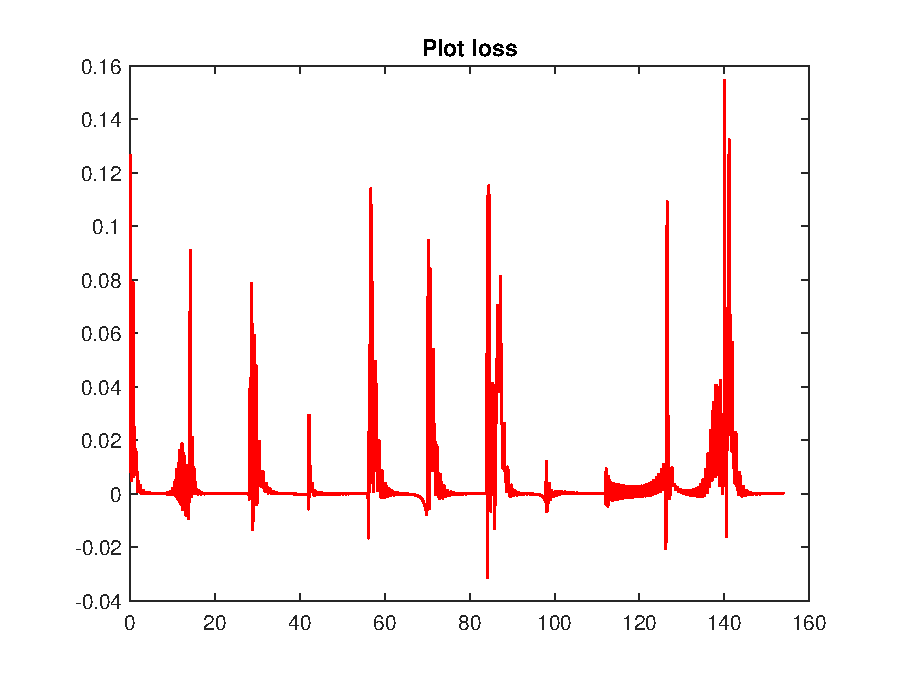
\includegraphics[width=9.5cm,height=4.5cm]{ch4/img/loss.eps}
    \caption{Evolution of the Loss Function during the simulation.}
    \label{fig:loss}
\end{figure}


%===============================
\section{Conclusion}\label{sec7}
This paper presented a robust hybrid estimation framework designed to address the challenges of vehicle motion tracking in the presence of unmodeled nonlinearities. We proposed a layered architecture that integrates a physics-based Generalized Unknown Input Observer (UIO) with a data-driven Neural Adaptive Observer. To overcome the structural limitations of standard observers, specifically when the rank condition $rank(CB) = rank(B)$ is not met, we introduced a regularization technique combined with an output-derivative based generalized model. This approach ensures the existence of the observer and provides a reliable initial estimate of the unknown dynamics. This estimate subsequently serves as a supervisor for a neural network, which refines the approximation of complex nonlinearities, such as variable tire-road friction, through online learning. Theoretical analysis demonstrated that the proposed method guarantees $\mathcal{H}^1$ and $\mathcal{L}^2$ stability for the estimation errors, provided that the derived Linear Matrix Inequality (LMI) conditions are satisfied. Future work will focus on the experimental validation of this framework using real driving data and its extension to discrete-time formulations for embedded implementation.
